\documentclass[12pt]{article}

\usepackage[utf8]{inputenc}
\usepackage[T1]{fontenc}
\usepackage[brazilian]{babel}
\usepackage{geometry}
\usepackage{hyperref}
\usepackage{graphicx}
\usepackage{subcaption}
\usepackage{xcolor}
\usepackage{titlesec}
\usepackage{enumitem}
\usepackage{booktabs}
\usepackage{float}
\usepackage{array}

\geometry{left=1.8cm, right=1.8cm, top=2cm, bottom=2cm}
\titlespacing*{\section}{0pt}{1.5ex plus 1ex minus .2ex}{1ex plus .2ex}
\titlespacing*{\subsection}{0pt}{1.2ex plus 1ex minus .2ex}{0.8ex plus .2ex}

\graphicspath{{figuras/}}

\title{Relatório de Progresso: Mineração de Padrões Frequentes \\ em Acidentes em Rodovias Federais}

\author{Erik Roberto Reis Neves, Gabriel Campos Prudente, Felipe Silva Fraga Damasceno}

\date{Maio de 2026}

\begin{document}

\maketitle

\begin{abstract}
Este relatório intermediário documenta o progresso do Grupo~18 no projeto de Mineração de Dados sobre acidentes em rodovias federais, utilizando dados abertos da Polícia Rodoviária Federal (PRF) com recorte geográfico em Minas Gerais. Descrevemos o refinamento dos objetivos, a fundamentação metodológica baseada em CRISP-DM, os resultados preliminares da análise exploratória, a infraestrutura de pipeline implementada e o plano de experimentos para as fases de modelagem e avaliação. Os resultados experimentais completos de mineração de regras de associação serão apresentados no relatório final.
\end{abstract}

\section{Introdução e Refinamento dos Objetivos}

Os acidentes de trânsito em rodovias federais representam um problema de saúde pública e infraestrutura no Brasil. A PRF registra sistematicamente essas ocorrências, gerando bases de dados ricas em variáveis temporais, ambientais, viárias e de consequência. Análises univariadas são insuficientes para capturar a interação simultânea de múltiplos fatores de risco; técnicas de mineração de dados permitem descobrir padrões ocultos e correlações não triviais.

\subsection{Objetivo Geral}

Desenvolver um estudo completo de Mineração de Dados sobre acidentes rodoviários federais, identificando \textbf{padrões ocultos e regras de associação estatisticamente relevantes} associadas à severidade dos acidentes.

\subsection{Objetivos Específicos Refinados}

Com base na proposta inicial e na análise exploratória conduzida, os objetivos foram refinados da seguinte forma:

\begin{enumerate}[leftmargin=*]
    \item Identificar conjuntos frequentes de itens que caracterizem cenários de risco elevado em Minas Gerais (MG), utilizando representação transacional one-hot.
    \item Gerar e analisar regras de associação com métricas de suporte, confiança, lift e conviction, priorizando padrões interpretáveis e não redundantes.
    \item Segmentar a base por clustering (K-Means) como etapa \textbf{complementar}, investigando diferenças estruturais entre contextos (urbano vs.\ rural, perfis viários distintos).
    \item Operacionalizar as diretrizes de IA responsável \textbf{Explicabilidade} e \textbf{Monitoramento e Avaliação} na seleção, apresentação e validação temporal das regras.
\end{enumerate}

\subsection{Escopo e Decisões de Recorte}

O recorte analítico concentra-se em Minas Gerais sobre a base \texttt{datatran2026\_agrupados\_por\_ocorrencia.csv}, em que cada registro corresponde a uma ocorrência única de acidente. Essa granularidade foi escolhida por ser a mais natural para a representação transacional exigida pelo FP-Growth, uma vez que cada linha pode ser tratada como uma transação composta por múltiplos itens categóricos. Após filtragem por UF, o conjunto analisado totaliza 2.985 ocorrências no período considerado.

Quanto aos métodos, o FP-Growth constitui a técnica principal para extração de itemsets frequentes e geração de regras de associação. O K-Means, por sua vez, será empregado de forma complementar como etapa de segmentação prévia, permitindo investigar se padrões locais --- por exemplo, em trechos urbanos versus rurais --- permanecem ocultos quando se analisa apenas a base global.

\section{Trabalhos Relacionados}

\subsection{Mineração de Padrões Frequentes}

Zaki e Meira Jr.\ \cite{zaki2020} descrevem o algoritmo FP-Growth e sua estrutura FP-Tree, que compacta a base transacional e evita a geração explícita de candidatos, sendo adequado para bases de alta dimensionalidade como a da PRF. Métricas clássicas --- suporte, confiança, lift e conviction --- são utilizadas para filtrar associações espúrias e priorizar padrões informativos.

\subsection{Metodologia CRISP-DM}

Wirth e Hipp \cite{wirth2000} propõem o CRISP-DM como processo padrão para projetos de mineração de dados, estruturando o trabalho em fases iterativas: compreensão do negócio e dos dados, preparação, modelagem, avaliação e deployment. Adotamos essa estrutura para organizar o pipeline em seis notebooks reprodutíveis, o que facilita o trabalho paralelo do grupo e o rastreamento de progresso por fase.

\subsection{Dados Abertos da PRF}

A Polícia Rodoviária Federal disponibiliza publicamente bases consolidadas de acidentes em rodovias federais \cite{prf2026}, com documentação sobre variáveis temporais, espaciais, ambientais e de gravidade. Essas bases têm sido utilizadas em estudos de segurança viária e análises descritivas, mas a aplicação sistemática de mineração de regras de associação multivariadas sobre recortes regionais permanece pouco explorada na literatura acadêmica do grupo.

\section{Descrição da Investigação}

\subsection{Problema e Questões de Pesquisa}

O problema central consiste em identificar \textbf{regras de associação estatisticamente significativas e não triviais} que relacionem combinações de fatores contextuais à ocorrência de acidentes de alta gravidade. Diferentemente de abordagens centradas em variáveis isoladas, buscamos padrões multivariados de coocorrência capazes de revelar estruturas latentes nos dados --- isto é, combinações recorrentes de condições ambientais, temporais e viárias que aparecem de forma conjunta nos registros, e não apenas correlações marginais entre atributos individuais.

Com base na análise exploratória (Fase~2), formulamos cinco hipóteses a serem investigadas na modelagem:

\begin{enumerate}[leftmargin=*]
    \item \textbf{H1}: Combinações de \{Plena Noite, Pista Simples, Zona Rural\} estão associadas a maior gravidade.
    \item \textbf{H2}: Finais de semana + Madrugada apresentam padrões distintos de associação.
    \item \textbf{H3}: Colisões frontais e atropelamentos têm lift elevado com acidentes fatais.
    \item \textbf{H4}: Condições meteorológicas adversas combinadas com tipo de pista influenciam a gravidade.
    \item \textbf{H5}: Padrões de acidentes variam entre zonas urbanas e rurais.
\end{enumerate}

A confirmação ou refutação dessas hipóteses mediante regras de associação será conduzida na fase de modelagem e reportada no relatório final.

\subsection{Dados PRF e Recorte Geográfico}

O projeto utiliza três arquivos CSV disponibilizados pela PRF (2026), selecionáveis por meio de um dicionário central no notebook de setup. A base por ocorrência (\texttt{datatran2026\_agrupados\_por\_ocorrencia.csv}) contém 30 colunas e cerca de 23.475 registros nacionais; a base por pessoa (\texttt{acidentes2026\_agrupados\_por\_pessoa.csv}) reúne 35 colunas e aproximadamente 64.125 registros, incluindo variáveis demográficas; e a base de todas causas e tipos (\texttt{acidentes2026\_todas\_causas\_tipos.csv}) expande multicausas em 37 colunas e cerca de 196.099 registros. Para este estudo, adotamos a granularidade por ocorrência como dataset principal.

Após aplicar o filtro geográfico UF = MG, obtivemos 2.985 ocorrências e 36 colunas analíticas. Na preparação transacional, selecionamos 12 atributos categóricos --- incluindo features engenheiradas como \texttt{faixa\_horaria} e \texttt{gravidade\_binaria} ---, o que produziu inicialmente 207 itens no formato one-hot \texttt{coluna=valor}. Para evitar a explosão de itens raros ou dominantes, aplicamos filtragem de frequência entre 1\% e 99\%, reduzindo o conjunto final a 83 itens válidos para mineração.

\subsection{Dicionário mínimo de variáveis (para leitura do relatório)}

Nesta seção, resumimos as variáveis centrais utilizadas na análise exploratória e que compõem os itens transacionais empregados na mineração:
\begin{itemize}[leftmargin=*]
    \item \texttt{classificacao\_acidente}: gravidade do acidente (``Sem Vítimas'', ``Com Vítimas Feridas'', ``Com Vítimas Fatais'').
    \item \texttt{tipo\_acidente}: categoria do evento (o \textit{que} ocorreu, por exemplo colisões, saída de leito carroçável, atropelamento).
    \item \texttt{causa\_acidente}: causa atribuída (o \textit{porquê} do evento segundo o registro, por exemplo ausência de reação, velocidade incompatível).
    \item \texttt{fase\_dia}: fase do dia (ex.: plena noite, amanhecer, pleno dia).
    \item \texttt{dia\_semana}: dia da semana da ocorrência.
    \item \texttt{condicao\_metereologica}: condição meteorológica (ex.: céu claro, chuva).
    \item \texttt{tipo\_pista}, \texttt{tracado\_via}, \texttt{sentido\_via}: características da via.
    \item \texttt{uso\_solo}: indicador binário do entorno da via no dataset de ocorrência (valores \texttt{Sim}/\texttt{Não}). Neste relatório, tratamos \texttt{Sim} como contexto \textit{urbano} e \texttt{Não} como contexto \textit{rural}, em linha com a leitura exploratória do grupo sobre a codificação do campo pela PRF.
    \item \texttt{faixa\_horaria}: discretização do horário em faixas (madrugada/manhã/tarde/noite), derivada de \texttt{horario}.
    \item \texttt{fim\_de\_semana}: indicador derivado de \texttt{dia\_semana}.
    \item \texttt{gravidade\_binaria}: indicador derivado para separar acidentes fatais vs.\ não fatais, usado para apoiar filtros e comparações.
\end{itemize}

\subsection{Resultados Preliminares da EDA}

A Tabela~\ref{tab:gravidade} resume a distribuição da variável-alvo. Observa-se um desbalanceamento marcante: apenas 7,1\% dos acidentes são classificados como fatais, enquanto a grande maioria (79,3\%) resulta em vítimas feridas. Esse perfil de classes impactará diretamente a calibração do suporte mínimo no FP-Growth, pois padrões associados à gravidade fatal tenderão a apresentar suportes mais baixos e exigirão atenção especial na interpretação dos resultados.

\begin{table}[H]
    \centering
    \caption{Distribuição da classificação de gravidade (MG, $n = 2.985$).}
    \label{tab:gravidade}
    \begin{tabular}{lc}
        \toprule
        \textbf{Classificação} & \textbf{Proporção} \\
        \midrule
        Com Vítimas Feridas & 79,3\% \\
        Sem Vítimas & 13,6\% \\
        Com Vítimas Fatais & 7,1\% \\
        \bottomrule
    \end{tabular}
\end{table}

A análise de associação entre variáveis categóricas e a gravidade, conduzida via Cramér's~V, indicou que \texttt{tipo\_acidente} ($V = 0{,}399$), \texttt{causa\_acidente} ($V = 0{,}325$) e \texttt{tracado\_via} ($V = 0{,}175$) são os atributos mais fortemente associados à classificação do acidente. Esses resultados reforçam a relevância de incluir tais variáveis na representação transacional e orientam a expectativa de que regras envolvendo tipologia e causa do evento tendam a ser mais informativas do que combinações puramente temporais ou geográficas.

\paragraph{Como ler os gráficos a seguir.}
Em gráficos \textbf{normalizados}, cada barra/linha representa uma categoria (por exemplo, um tipo de acidente) e soma 100\%. Esses gráficos permitem comparar \textit{composição} de gravidade entre categorias, mas não substituem análises de volume (frequências absolutas). Em todas as interpretações, enfatizamos que associação estatística não implica causalidade.

\begin{figure}[H]
    \centering
    \begin{subfigure}[b]{0.48\textwidth}
        
\includegraphics[width=\textwidth]{distribuicao_gravidade.png}
        \caption{Distribuição de gravidade.}
        \label{fig:gravidade}
    \end{subfigure}
    \hfill
    \begin{subfigure}[b]{0.48\textwidth}
        
\includegraphics[width=\textwidth]{heatmap_temporal.png}
        \caption{Heatmap temporal (gravidade $\times$ dia $\times$ fase).}
        \label{fig:heatmap}
    \end{subfigure}
    \caption{Resultados preliminares da análise exploratória.}
    \label{fig:eda}
\end{figure}

\subsubsection*{Tipos de acidente (Top 10 + Outros)}

A Tabela~\ref{tab:top_tipos} lista os tipos de acidente mais frequentes no recorte (MG). A Figura~\ref{fig:top_tipos} mostra a distribuição absoluta, enquanto a Figura~\ref{fig:tipos_norm} mostra a composição de gravidade \textbf{normalizada} por tipo, evidenciando como a proporção de fatalidade varia entre categorias.

\begin{table}
\caption{Top tipos de acidente (MG).}
\label{tab:top_tipos}
\begin{tabular}{lrr}
\toprule
Tipo & Frequência & \% \\
\midrule
Saída de leito carroçável & 628 & 0.210 \\
Colisão traseira & 518 & 0.174 \\
Tombamento & 323 & 0.108 \\
Colisão transversal & 278 & 0.093 \\
Colisão com objeto & 261 & 0.087 \\
Colisão lateral mesmo sentido & 259 & 0.087 \\
Colisão frontal & 194 & 0.065 \\
Atropelamento de Pedestre & 116 & 0.039 \\
Incêndio & 87 & 0.029 \\
Queda de ocupante de veículo & 86 & 0.029 \\
Outros & 235 & 0.079 \\
\bottomrule
\end{tabular}
\end{table}


\begin{figure}[H]
    \centering
    \begin{subfigure}[b]{0.49\textwidth}
        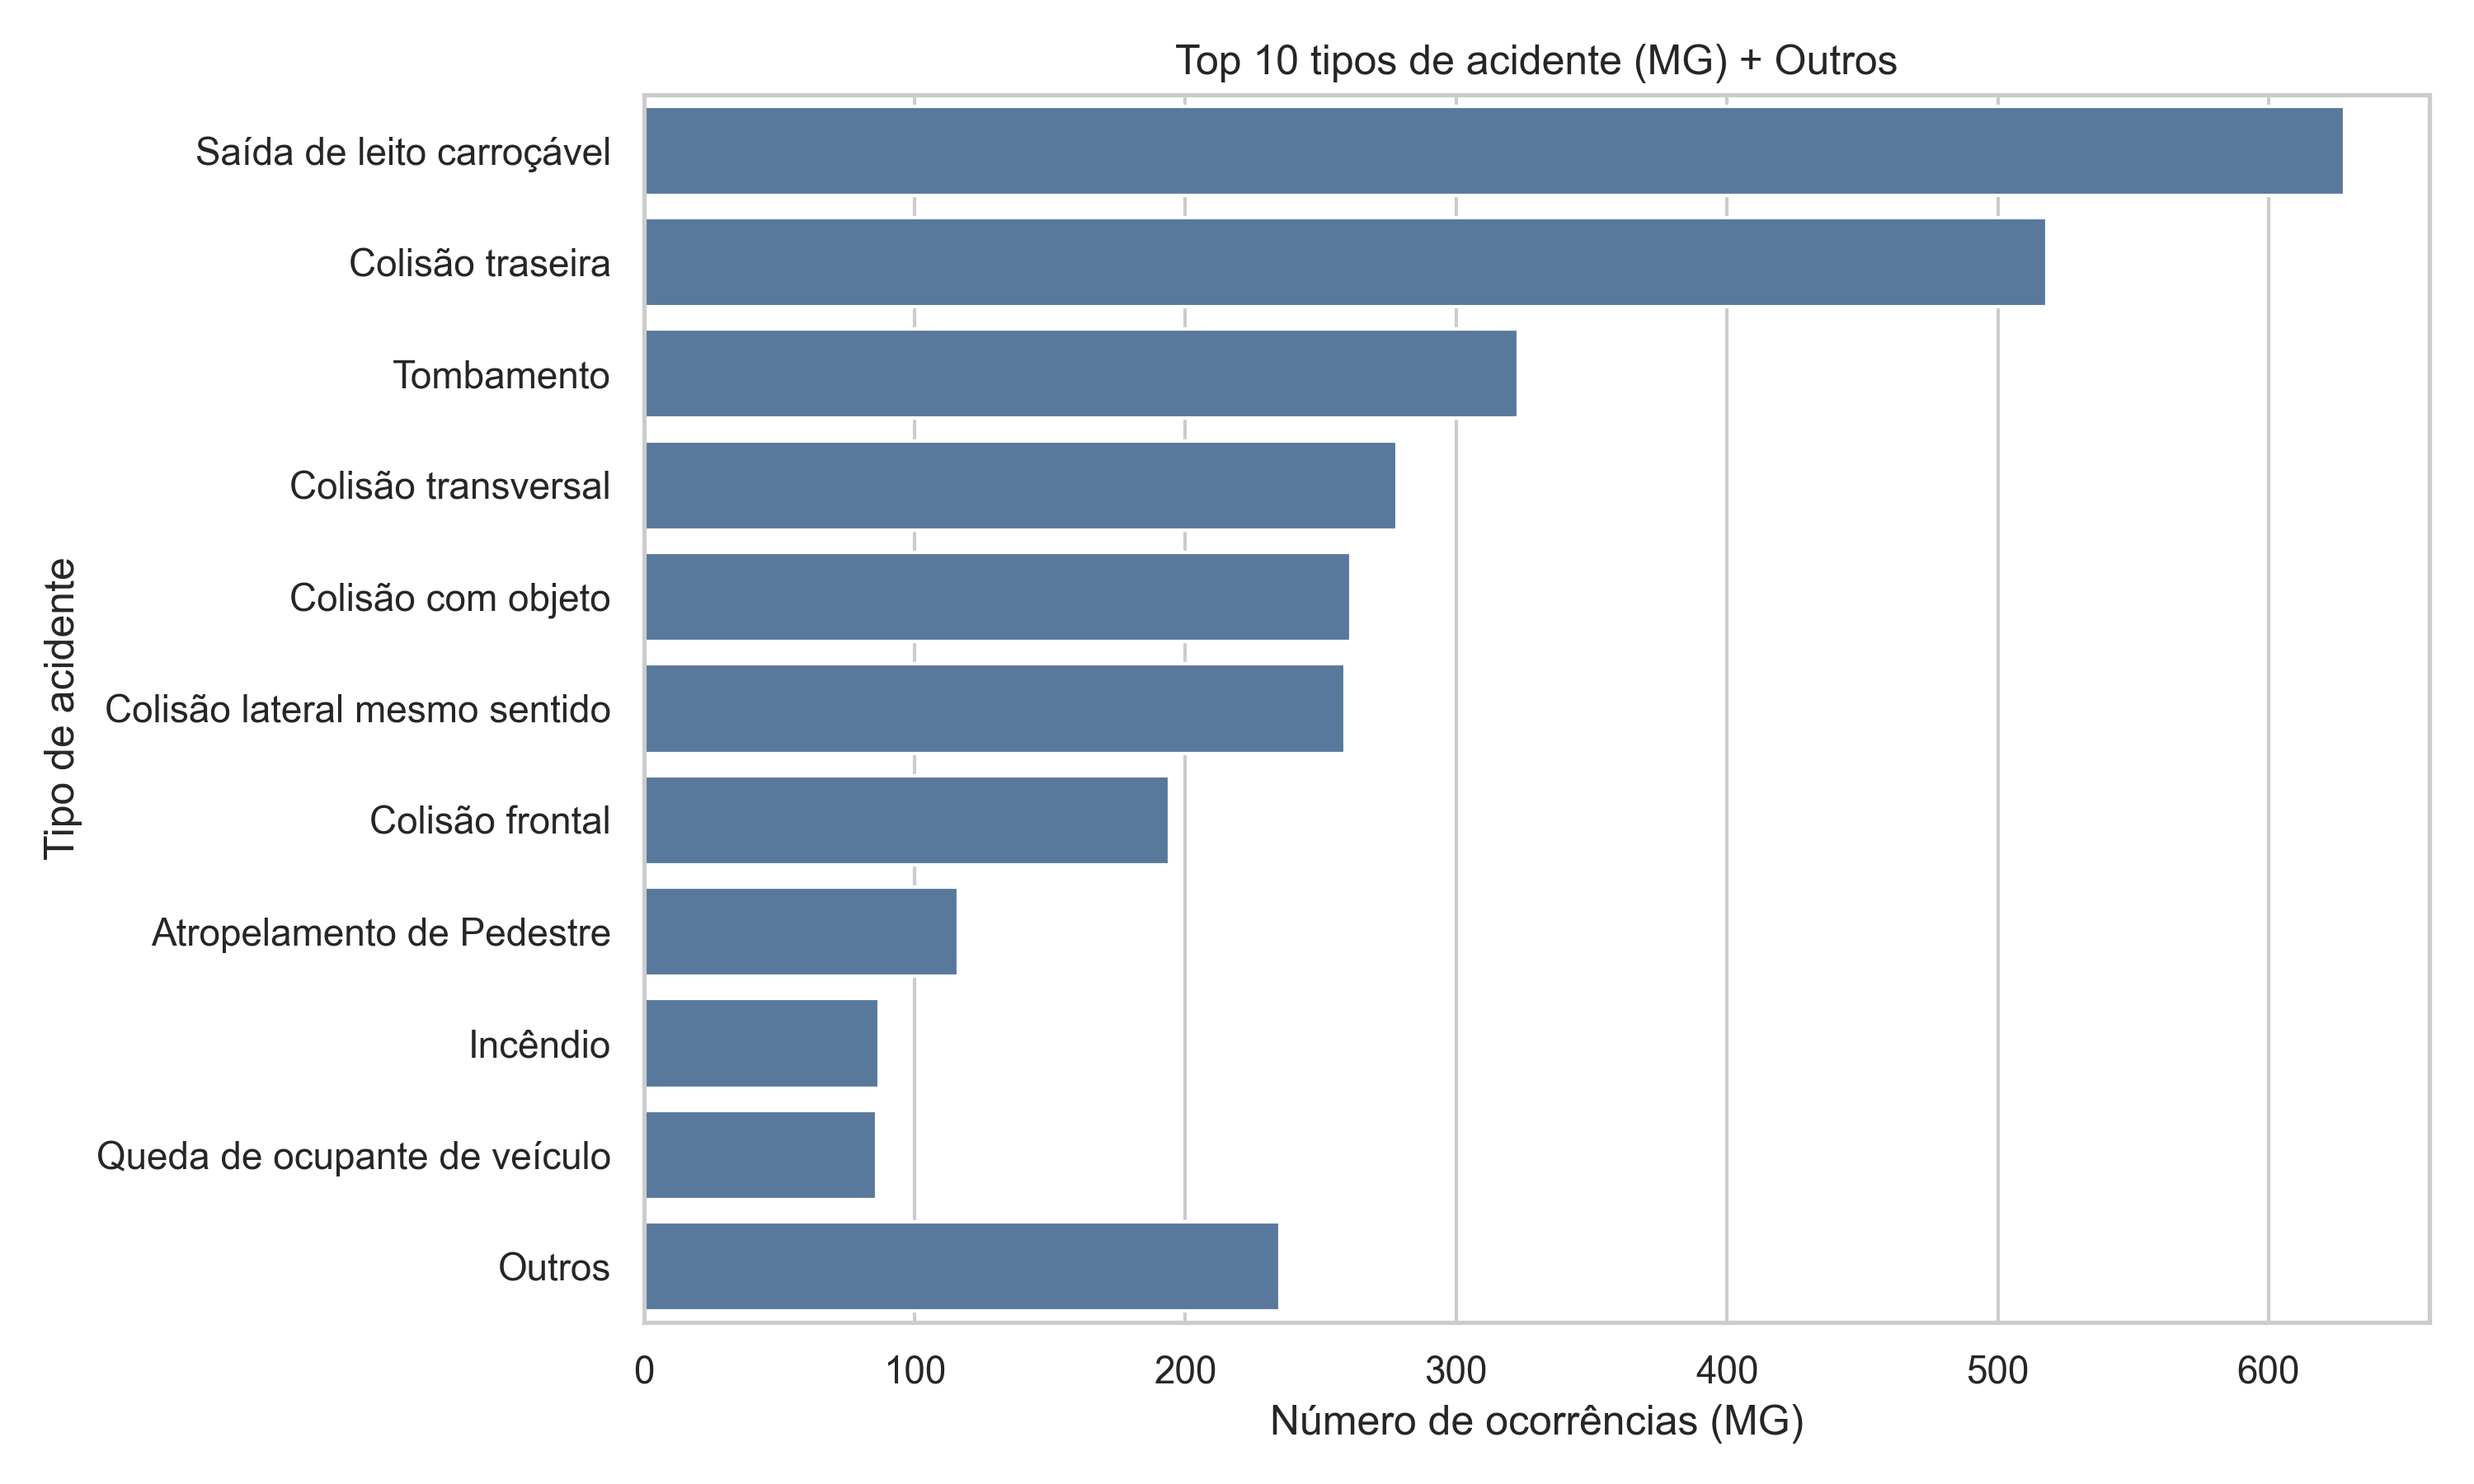
\includegraphics[width=\textwidth]{top_tipos_acidente.png}
        \caption{Top tipos (frequência).}
        \label{fig:top_tipos}
    \end{subfigure}
    \hfill
    \begin{subfigure}[b]{0.49\textwidth}
        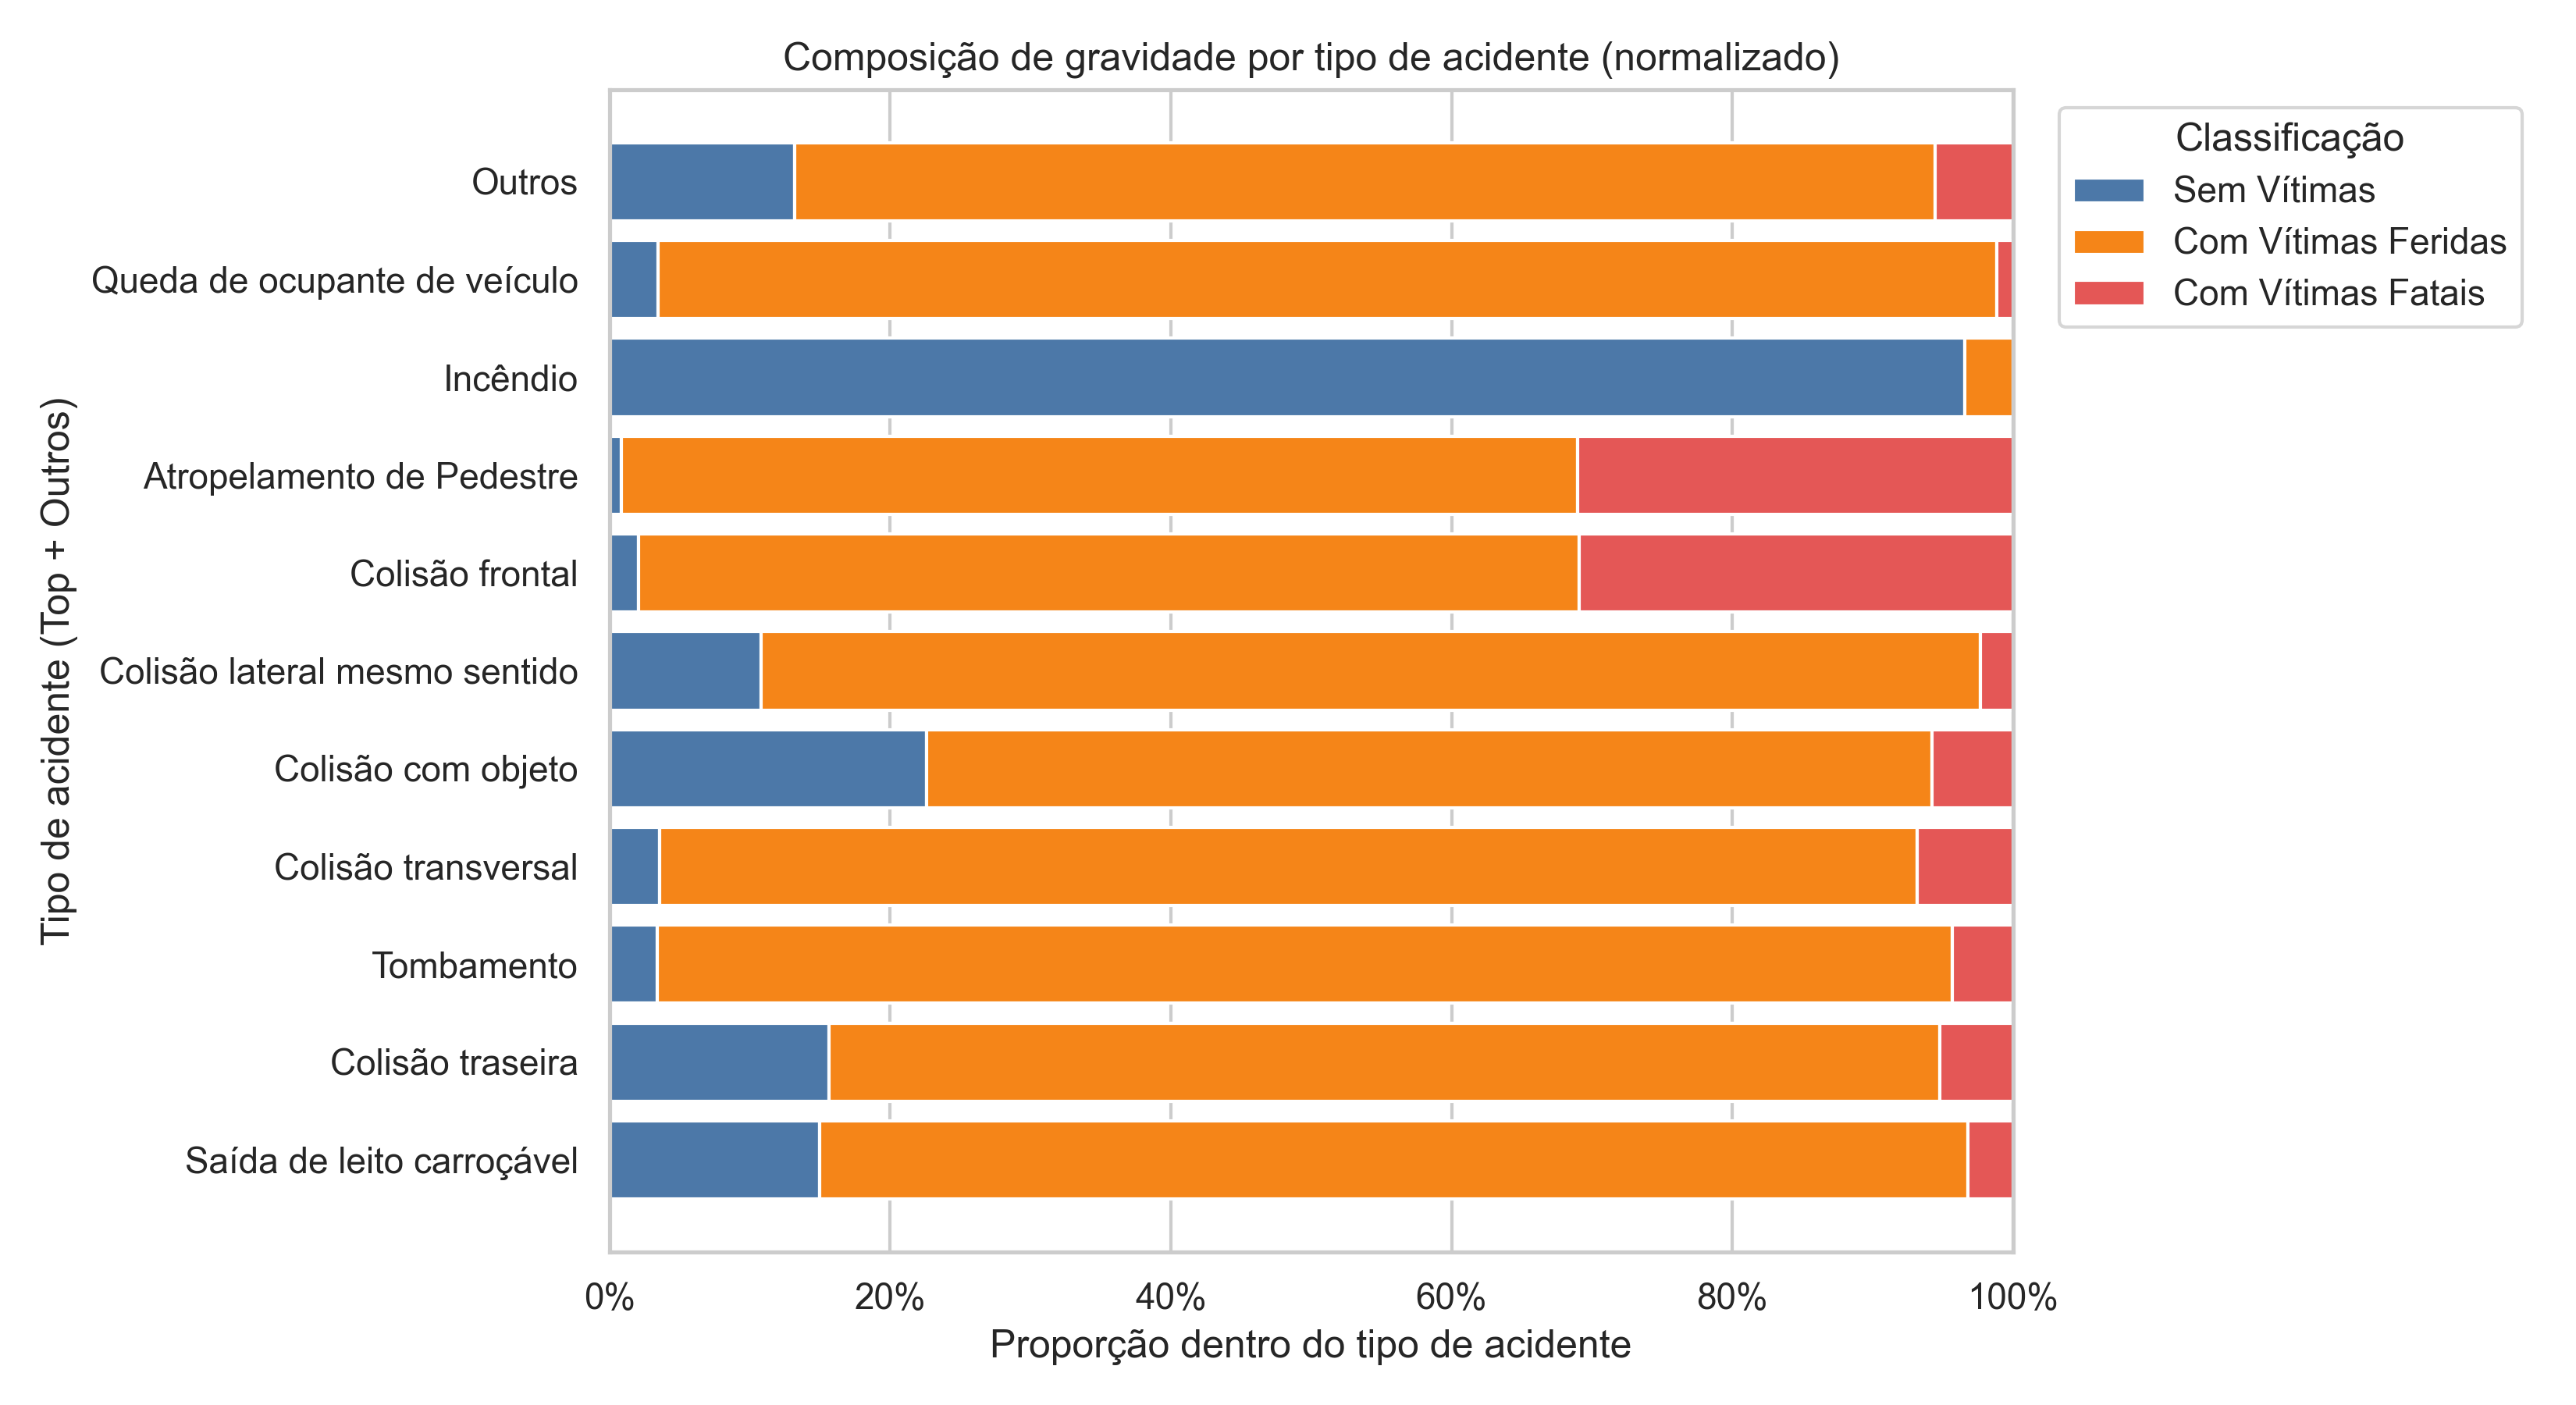
\includegraphics[width=\textwidth]{tipos_acidente_por_gravidade_norm.png}
        \caption{Gravidade por tipo (normalizado).}
        \label{fig:tipos_norm}
    \end{subfigure}
    \caption{Tipos de acidente no recorte MG (Top 10 + Outros).}
    \label{fig:tipos}
\end{figure}

\subsubsection*{Causas do acidente (Top 12 + Outros)}

Complementarmente, analisamos \texttt{causa\_acidente}, que representa a causa atribuída no registro (diferente do \textit{tipo} do evento). A Tabela~\ref{tab:top_causas} sumariza as causas mais frequentes, e a Figura~\ref{fig:causas_norm} apresenta a composição de gravidade normalizada por causa.

\begin{table}
\caption{Top causas de acidente (MG).}
\label{tab:top_causas}
\begin{tabular}{lrr}
\toprule
Causa & Frequência & \% \\
\midrule
Ausência de reação do condutor & 505 & 0.169 \\
Reação tardia ou ineficiente do condutor & 385 & 0.129 \\
Velocidade Incompatível & 355 & 0.119 \\
Acessar a via sem observar a presença dos outros veículos & 206 & 0.069 \\
Demais falhas mecânicas ou elétricas & 160 & 0.054 \\
Condutor Dormindo & 150 & 0.050 \\
Condutor deixou de manter distância do veículo da frente & 149 & 0.050 \\
Chuva & 117 & 0.039 \\
Ingestão de álcool pelo condutor & 98 & 0.033 \\
Manobra de mudança de faixa & 87 & 0.029 \\
Transitar na contramão & 79 & 0.026 \\
Ultrapassagem Indevida & 66 & 0.022 \\
Outros & 628 & 0.210 \\
\bottomrule
\end{tabular}
\end{table}


\begin{figure}[H]
    \centering
    \begin{subfigure}[b]{0.49\textwidth}
        
\includegraphics[width=\textwidth]{top_causas_gravidade.png}
        \caption{Causas por gravidade (visão absoluta).}
        \label{fig:causas_abs}
    \end{subfigure}
    \hfill
    \begin{subfigure}[b]{0.49\textwidth}
        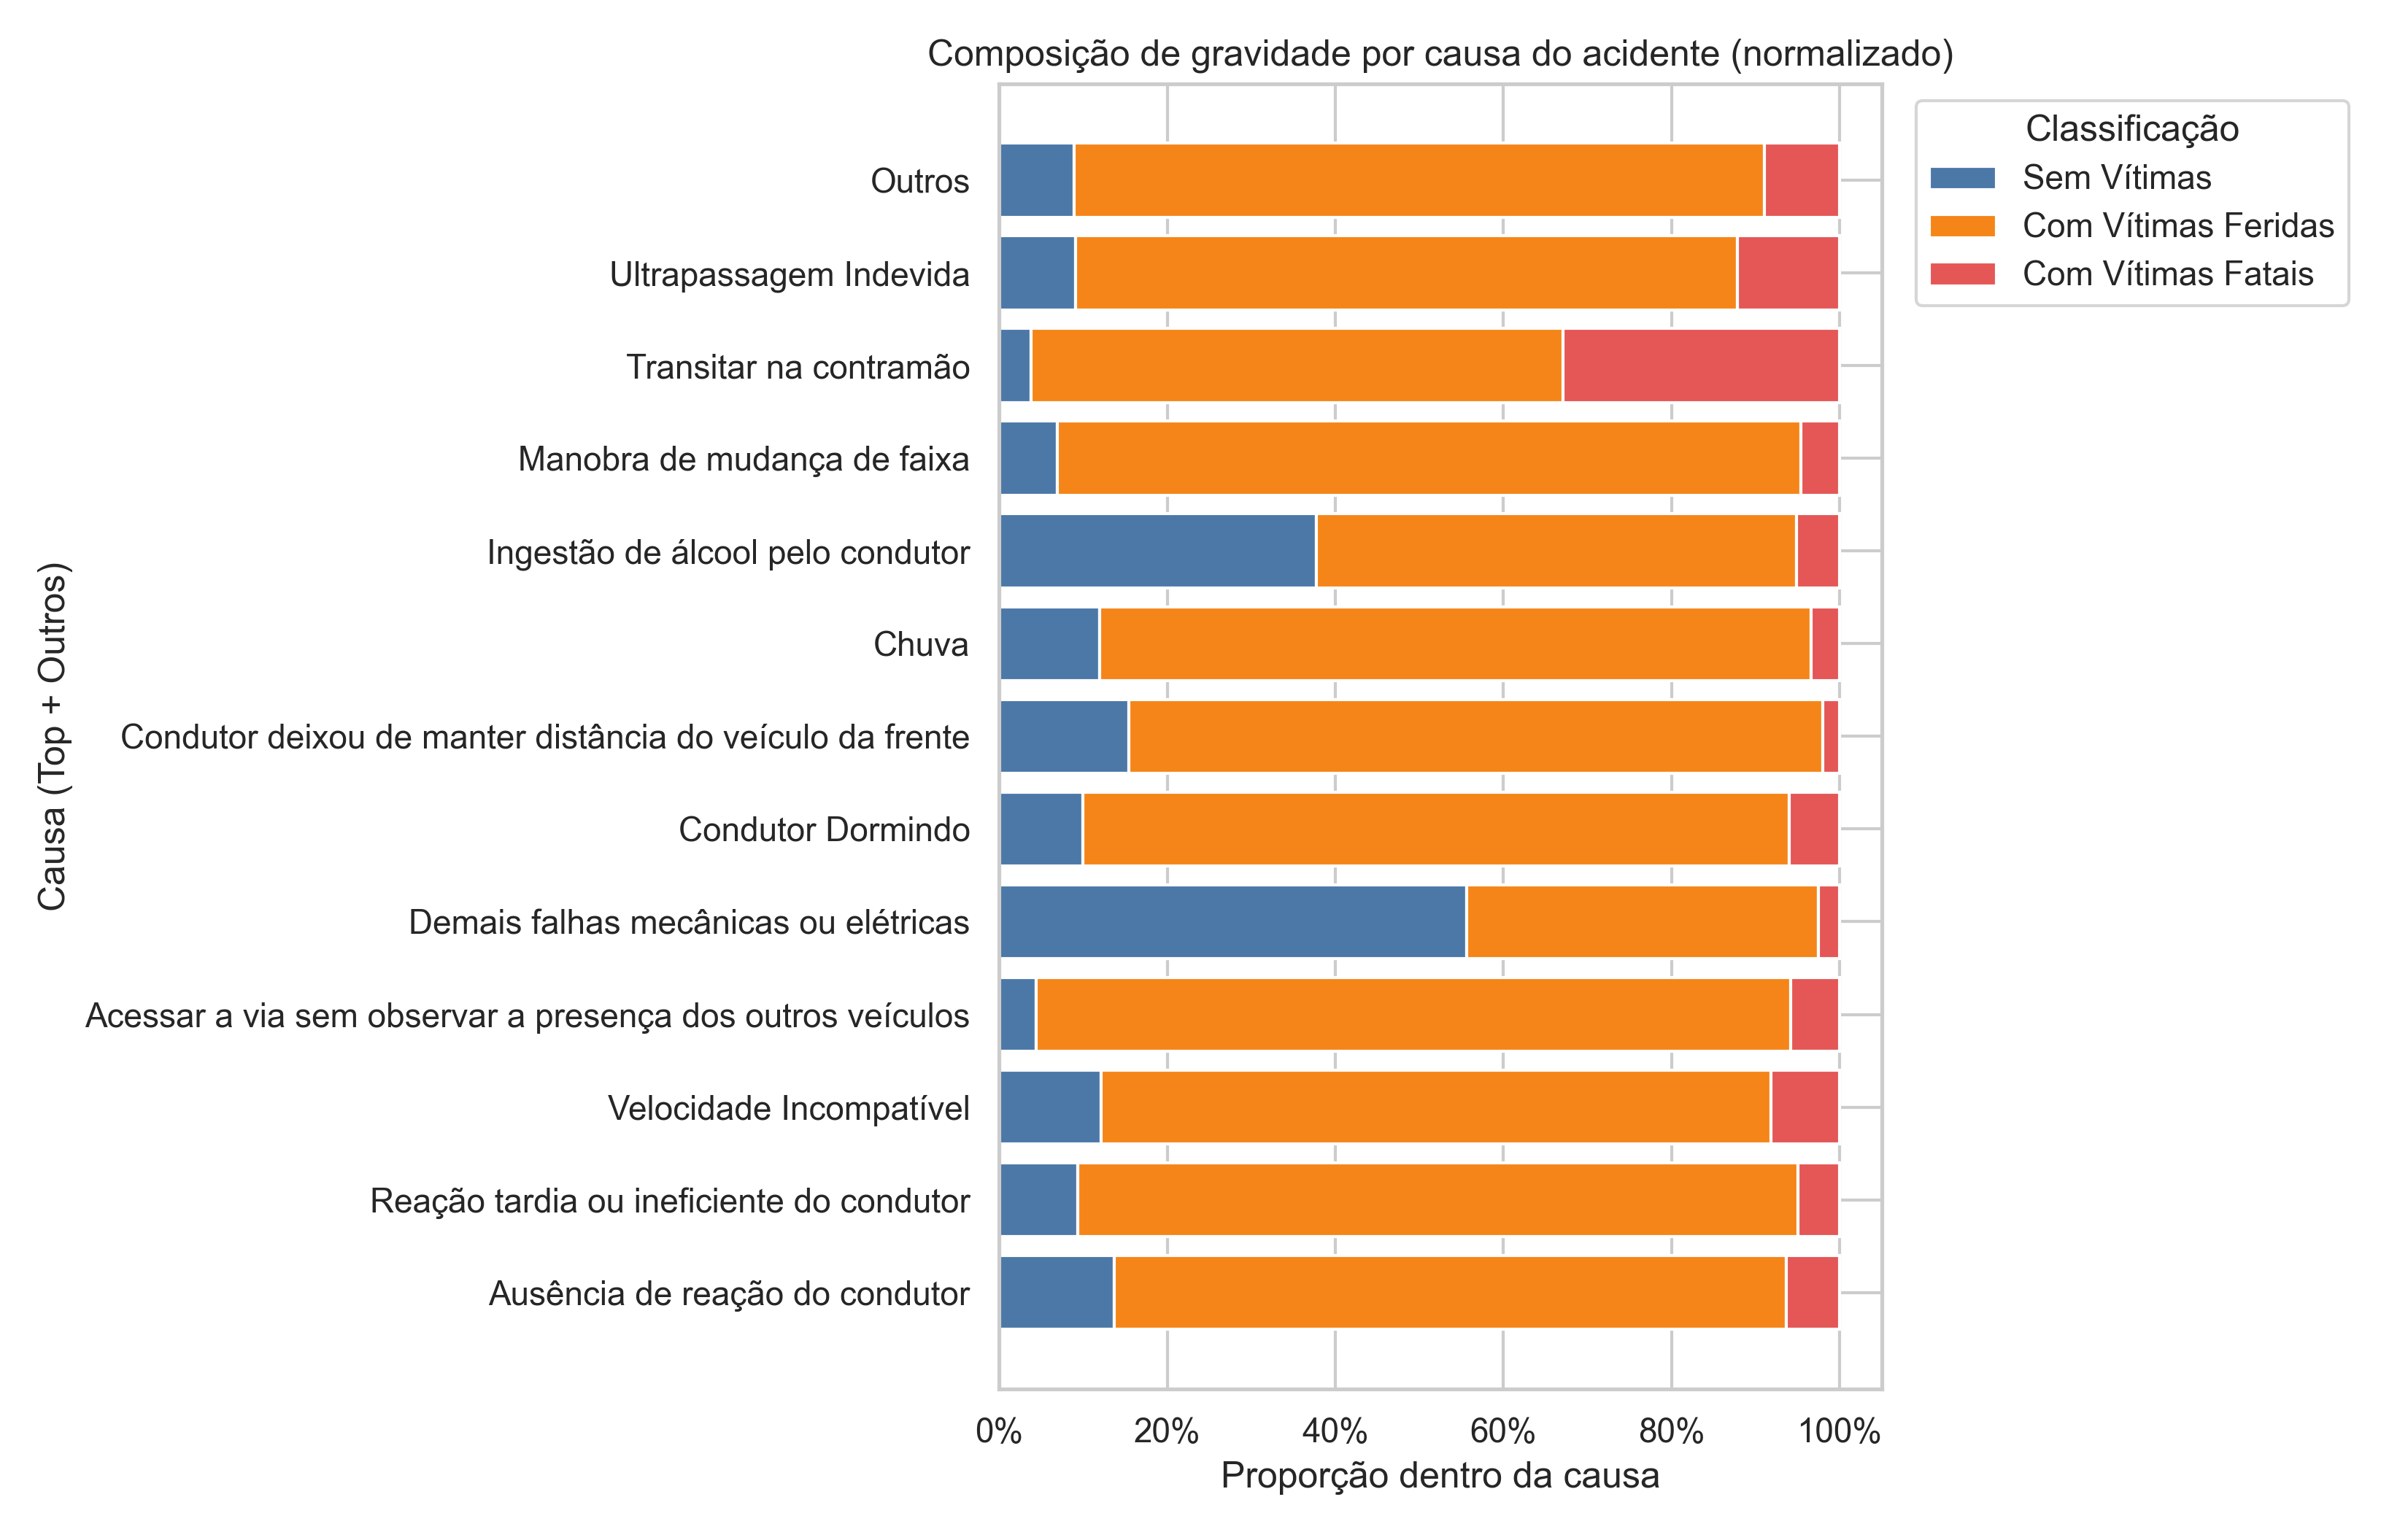
\includegraphics[width=\textwidth]{causas_por_gravidade_norm.png}
        \caption{Gravidade por causa (normalizado).}
        \label{fig:causas_norm}
    \end{subfigure}
    \caption{Causas do acidente no recorte MG (Top 12 + Outros).}
    \label{fig:causas}
\end{figure}

\subsubsection*{Condições de via e perfil temporal}

A Figura~\ref{fig:tipo_pista_heat} resume como a composição de gravidade varia entre os tipos de pista mais frequentes, enquanto a Figura~\ref{fig:heat_fatal} mostra o percentual de acidentes fatais em janelas \texttt{dia\_semana} $\times$ \texttt{fase\_dia}, permitindo comparar \textit{risco relativo} de fatalidade sem confundir com volume total de ocorrências.

\begin{figure}[H]
    \centering
    \begin{subfigure}[b]{0.49\textwidth}
        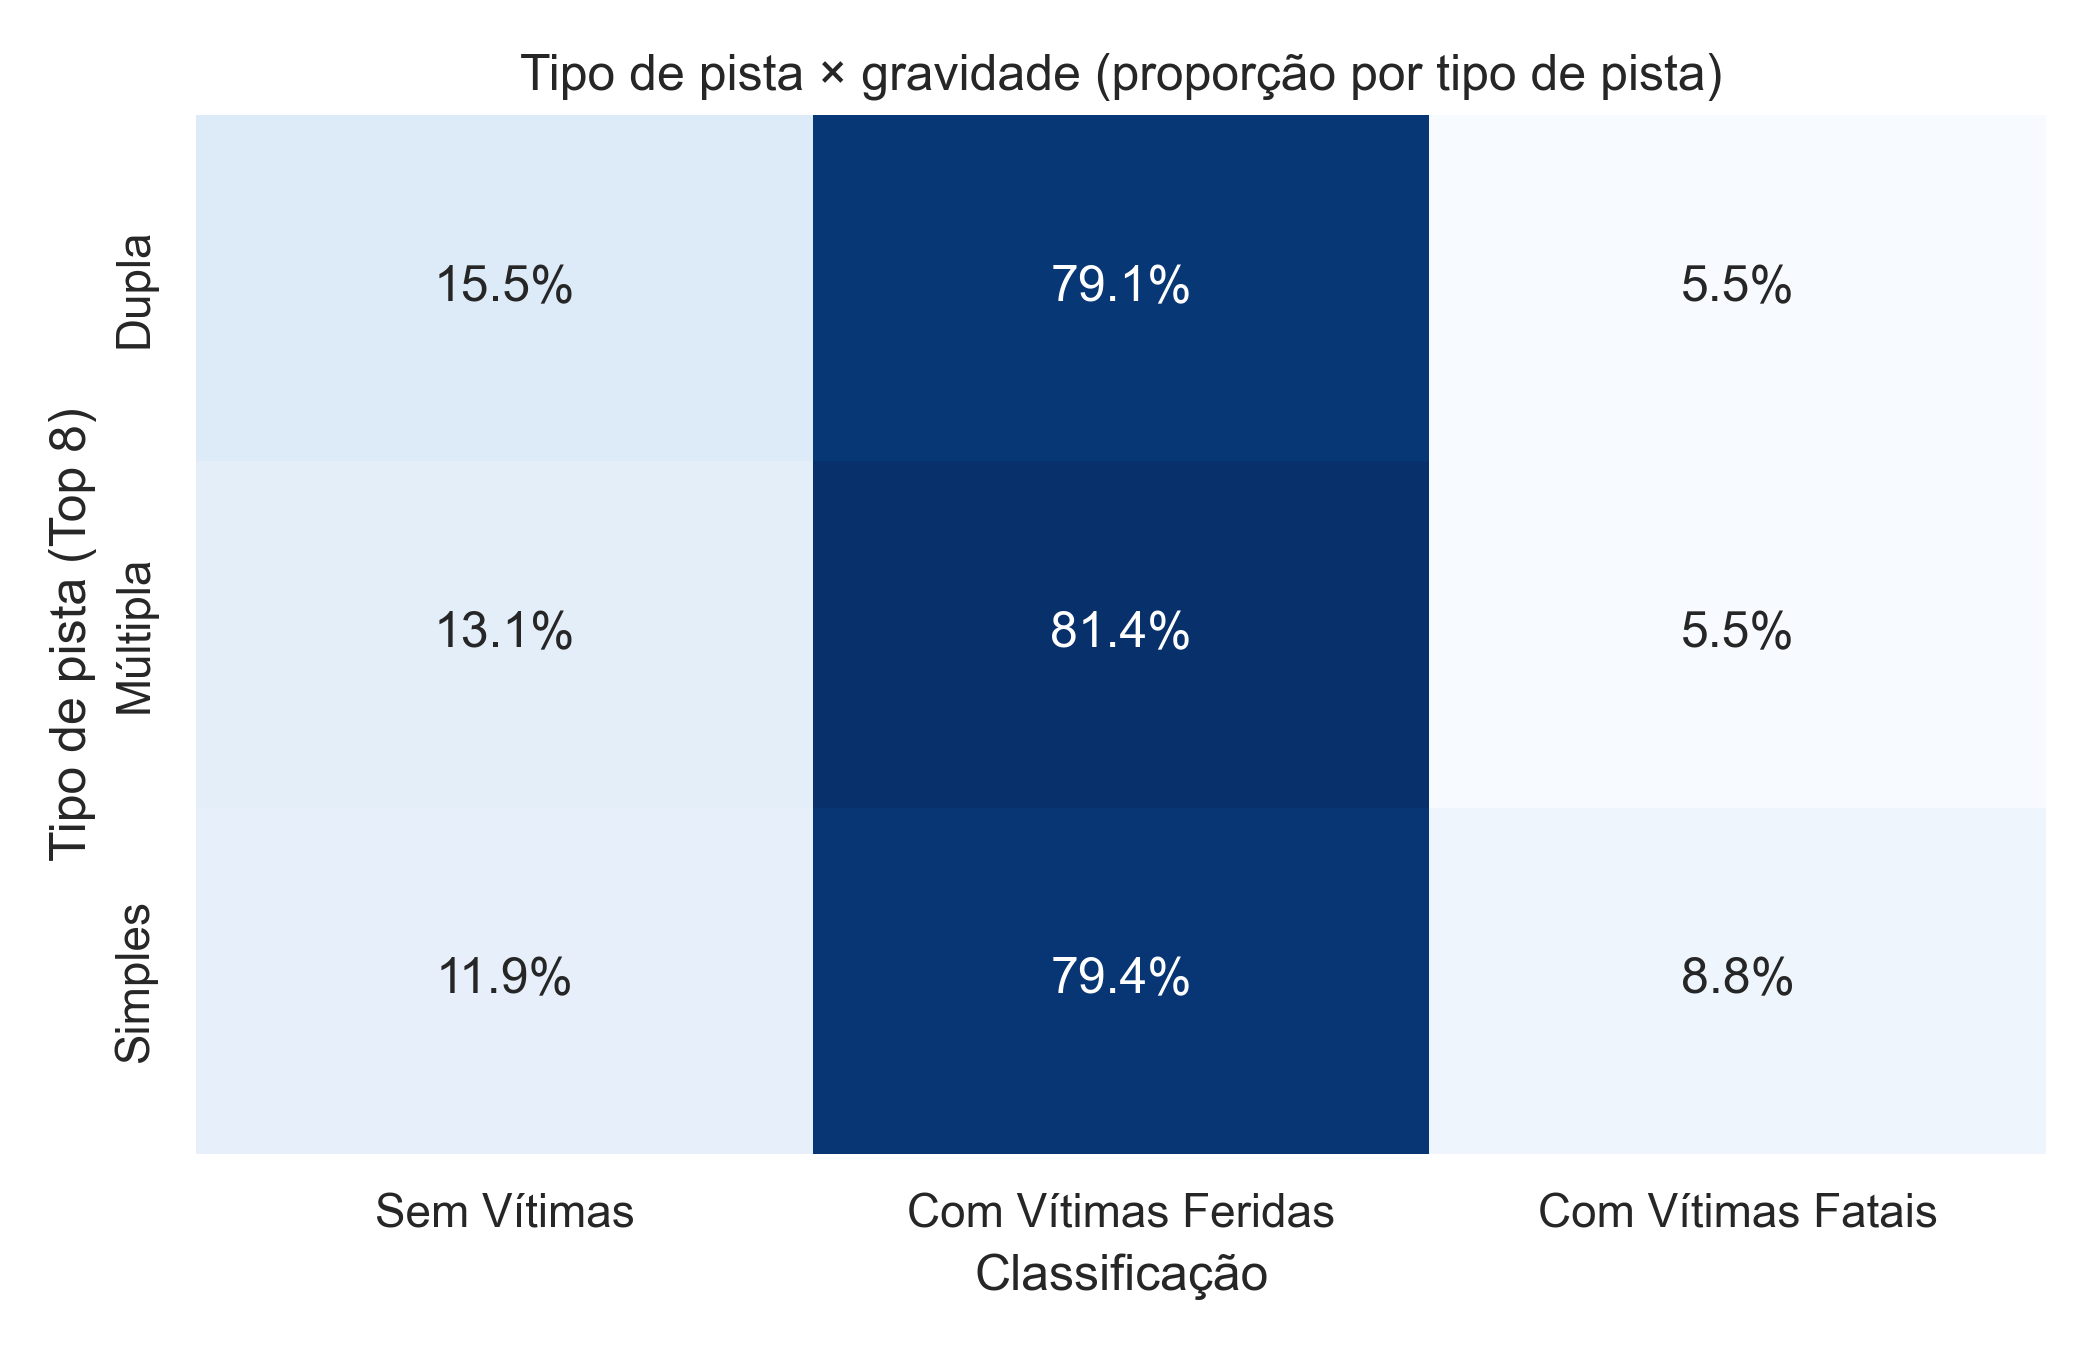
\includegraphics[width=\textwidth]{tipo_pista_x_gravidade_heatmap.png}
        \caption{Tipo de pista $\times$ gravidade (proporção).}
        \label{fig:tipo_pista_heat}
    \end{subfigure}
    \hfill
    \begin{subfigure}[b]{0.49\textwidth}
        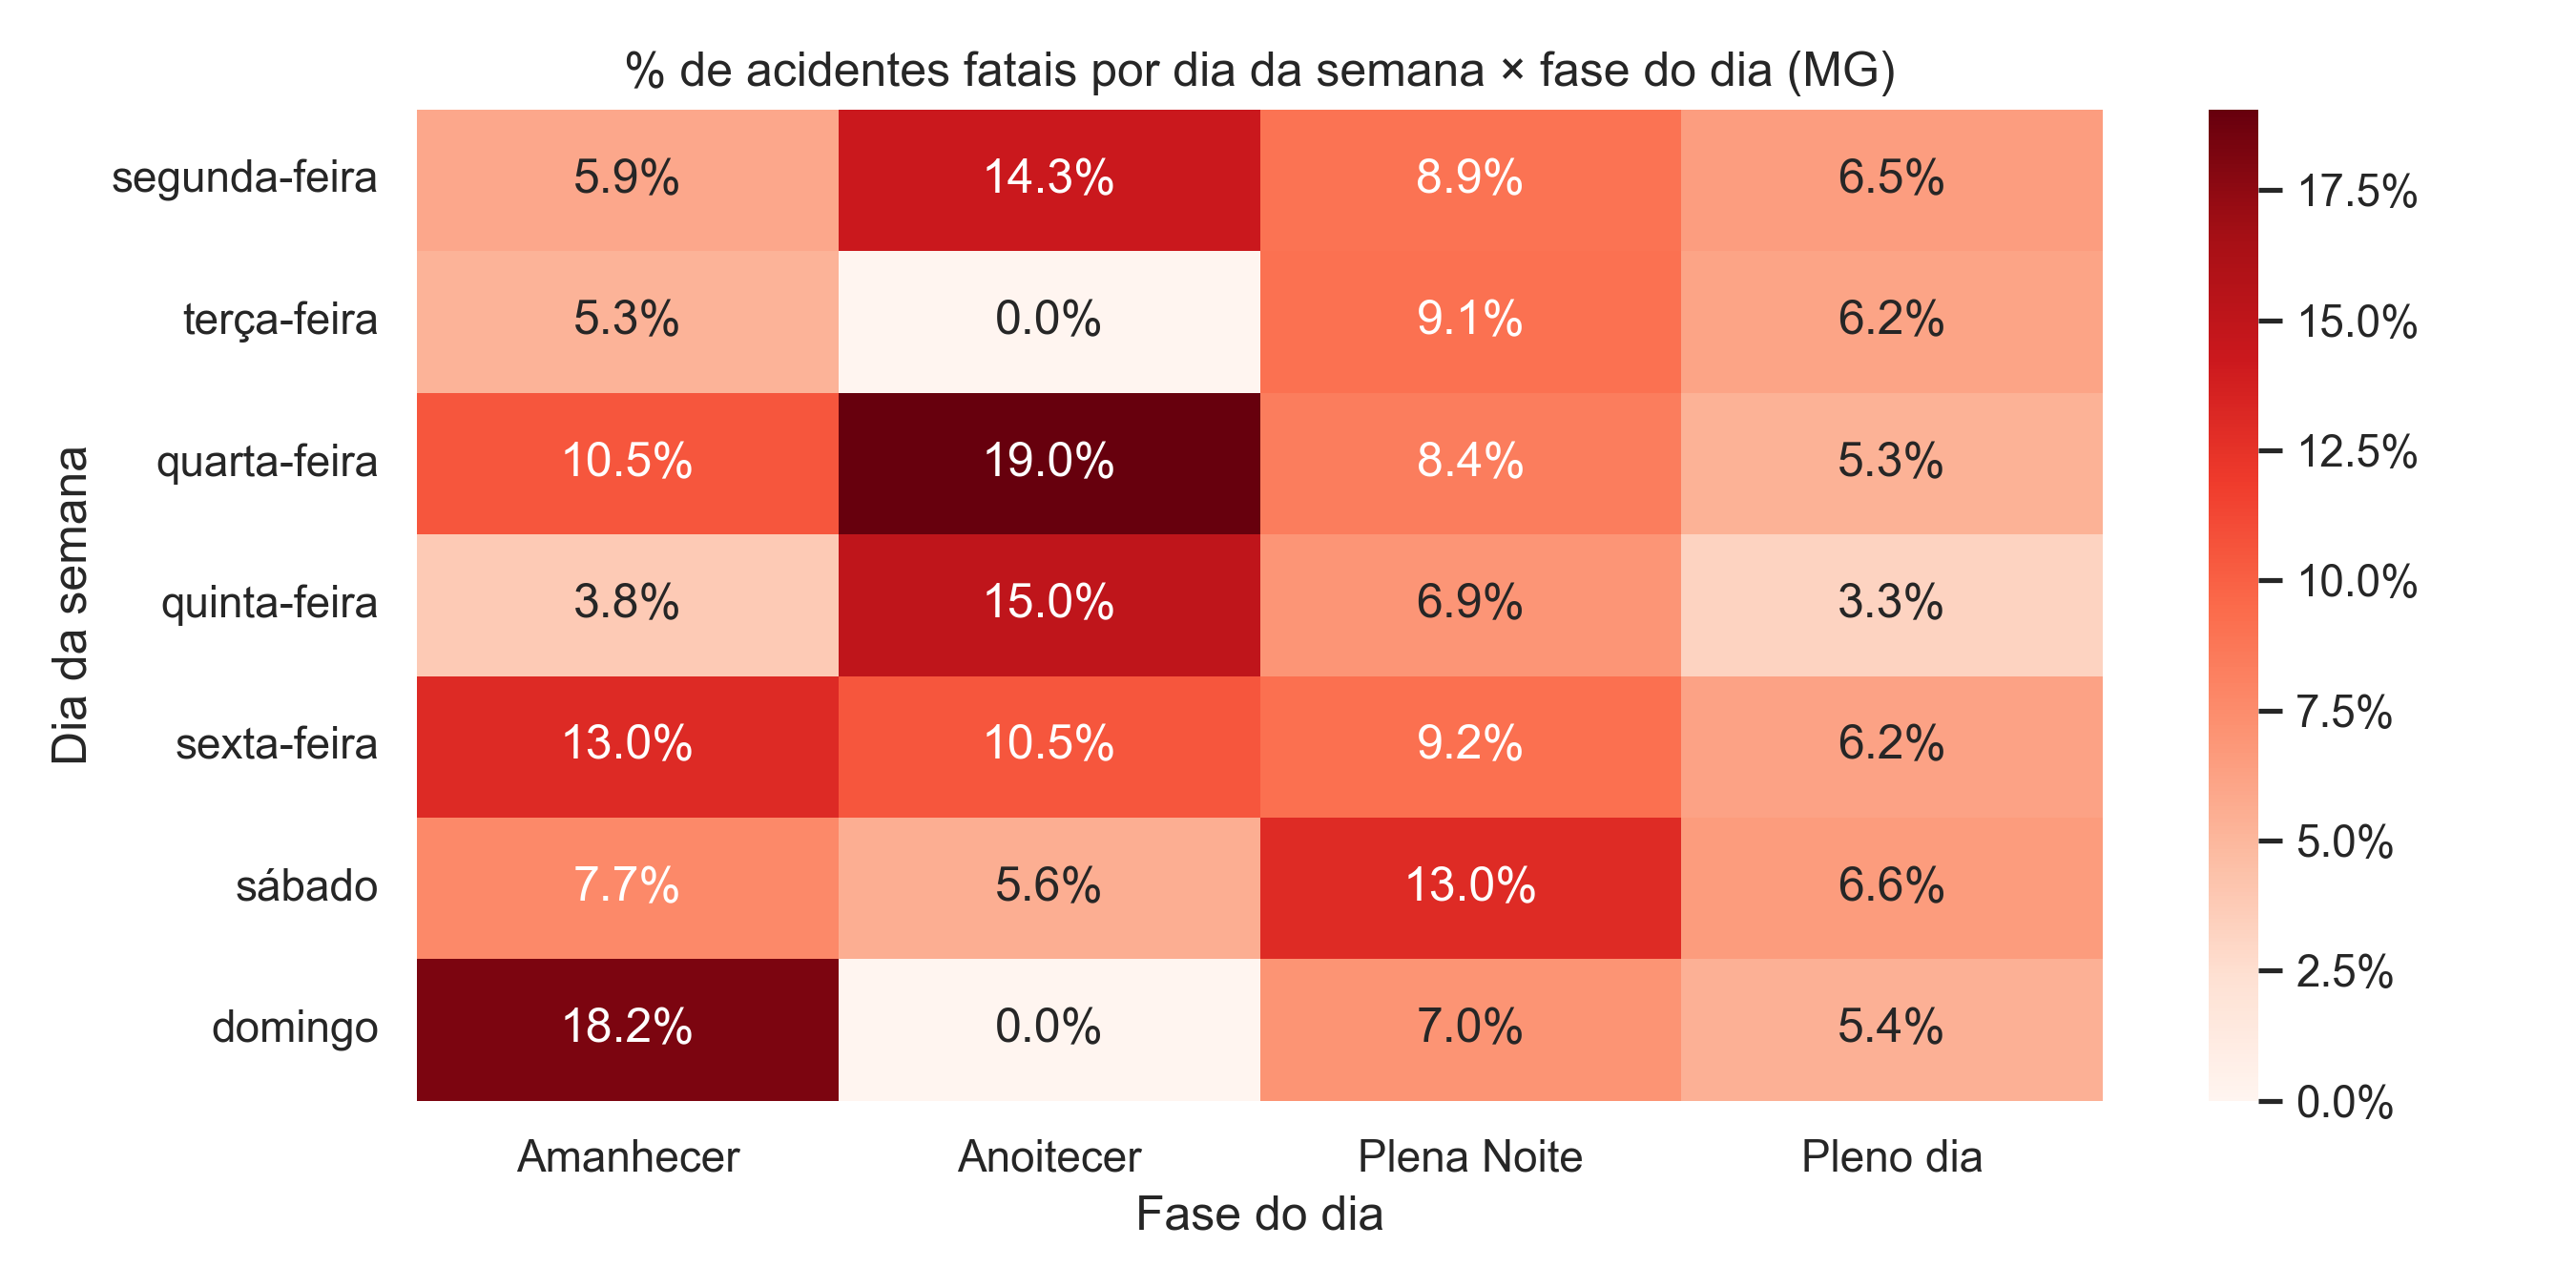
\includegraphics[width=\textwidth]{heatmap_percentual_fatais_temporal.png}
        \caption{\% de fatais por dia $\times$ fase do dia.}
        \label{fig:heat_fatal}
    \end{subfigure}
    \caption{Condições de via e perfil temporal no recorte MG.}
    \label{fig:via_tempo}
\end{figure}

Foram produzidas 17 visualizações exploratórias no notebook~02, abrangendo distribuições temporais, geográficas, categóricas e correlações entre variáveis numéricas. Conjuntamente, esses achados subsidiam a seleção de atributos transacionais, a calibragem de parâmetros de mineração e a formulação das hipóteses H1--H5 descritas acima.

\section{Metodologia Detalhada (CRISP-DM)}

O pipeline do projeto foi organizado em seis notebooks sequenciais, alinhados às fases do CRISP-DM. A configuração global --- caminhos, dataset ativo, filtros e seleção de colunas --- concentra-se no notebook \texttt{01\_setup\_e\_carregamento.ipynb} e é reutilizada pelos demais, garantindo consistência e permitindo trocar granularidade ou recorte geográfico alterando apenas constantes centrais, sem reescrever a lógica de cada etapa.

A Tabela~\ref{tab:config_global} resume os parâmetros de configuração adotados na execução atual do pipeline.

\begin{table}[H]
    \centering
    \caption{Configuração global do pipeline (notebooks 01 e 03).}
    \label{tab:config_global}
    \small
    \begin{tabular}{@{}p{3.6cm}p{9.8cm}@{}}
        \toprule
        \textbf{Parâmetro} & \textbf{Valor / descrição} \\
        \midrule
        \texttt{ACTIVE\_DATASET} &
        \texttt{por\_ocorrencia} $\rightarrow$ \texttt{datatran2026\_agrupados\_por\_ocorrencia.csv} \\
        \texttt{FILTRO\_UF} & \texttt{MG} \\
        \texttt{SEP} / \texttt{ENCODING} & \texttt{;} / \texttt{latin-1} (ISO-8859-1) \\
        \texttt{DATA\_DIR} & \texttt{../data/} \\
        \texttt{PROCESSED\_DIR} & \texttt{../data/processed/} \\
        \texttt{OUTPUT\_DIR} & \texttt{../outputs/} \\
        \texttt{COLUNAS\_CATEGORICAS\_COMUNS} &
        \texttt{dia\_semana}, \texttt{causa\_acidente}, \texttt{tipo\_acidente}, \texttt{classificacao\_acidente}, \texttt{fase\_dia}, \texttt{sentido\_via}, \texttt{condicao\_metereologica}, \texttt{tipo\_pista}, \texttt{tracado\_via}, \texttt{uso\_solo} \\
        \texttt{COLUNAS\_TRANSACIONAIS} &
        12 colunas: 10 categóricas comuns + \texttt{faixa\_horaria}, \texttt{fim\_de\_semana}, \texttt{gravidade\_binaria} \\
        Filtro de itens & frequência $\in [1\%,\; 99\%]$ $\rightarrow$ 207 itens $\rightarrow$ 83 itens finais \\
        \bottomrule
    \end{tabular}
\end{table}

A Figura~\ref{fig:pipeline} apresenta o fluxo de dados entre os notebooks e os artefatos intermediários gerados.

\begin{figure}[H]
    \centering
    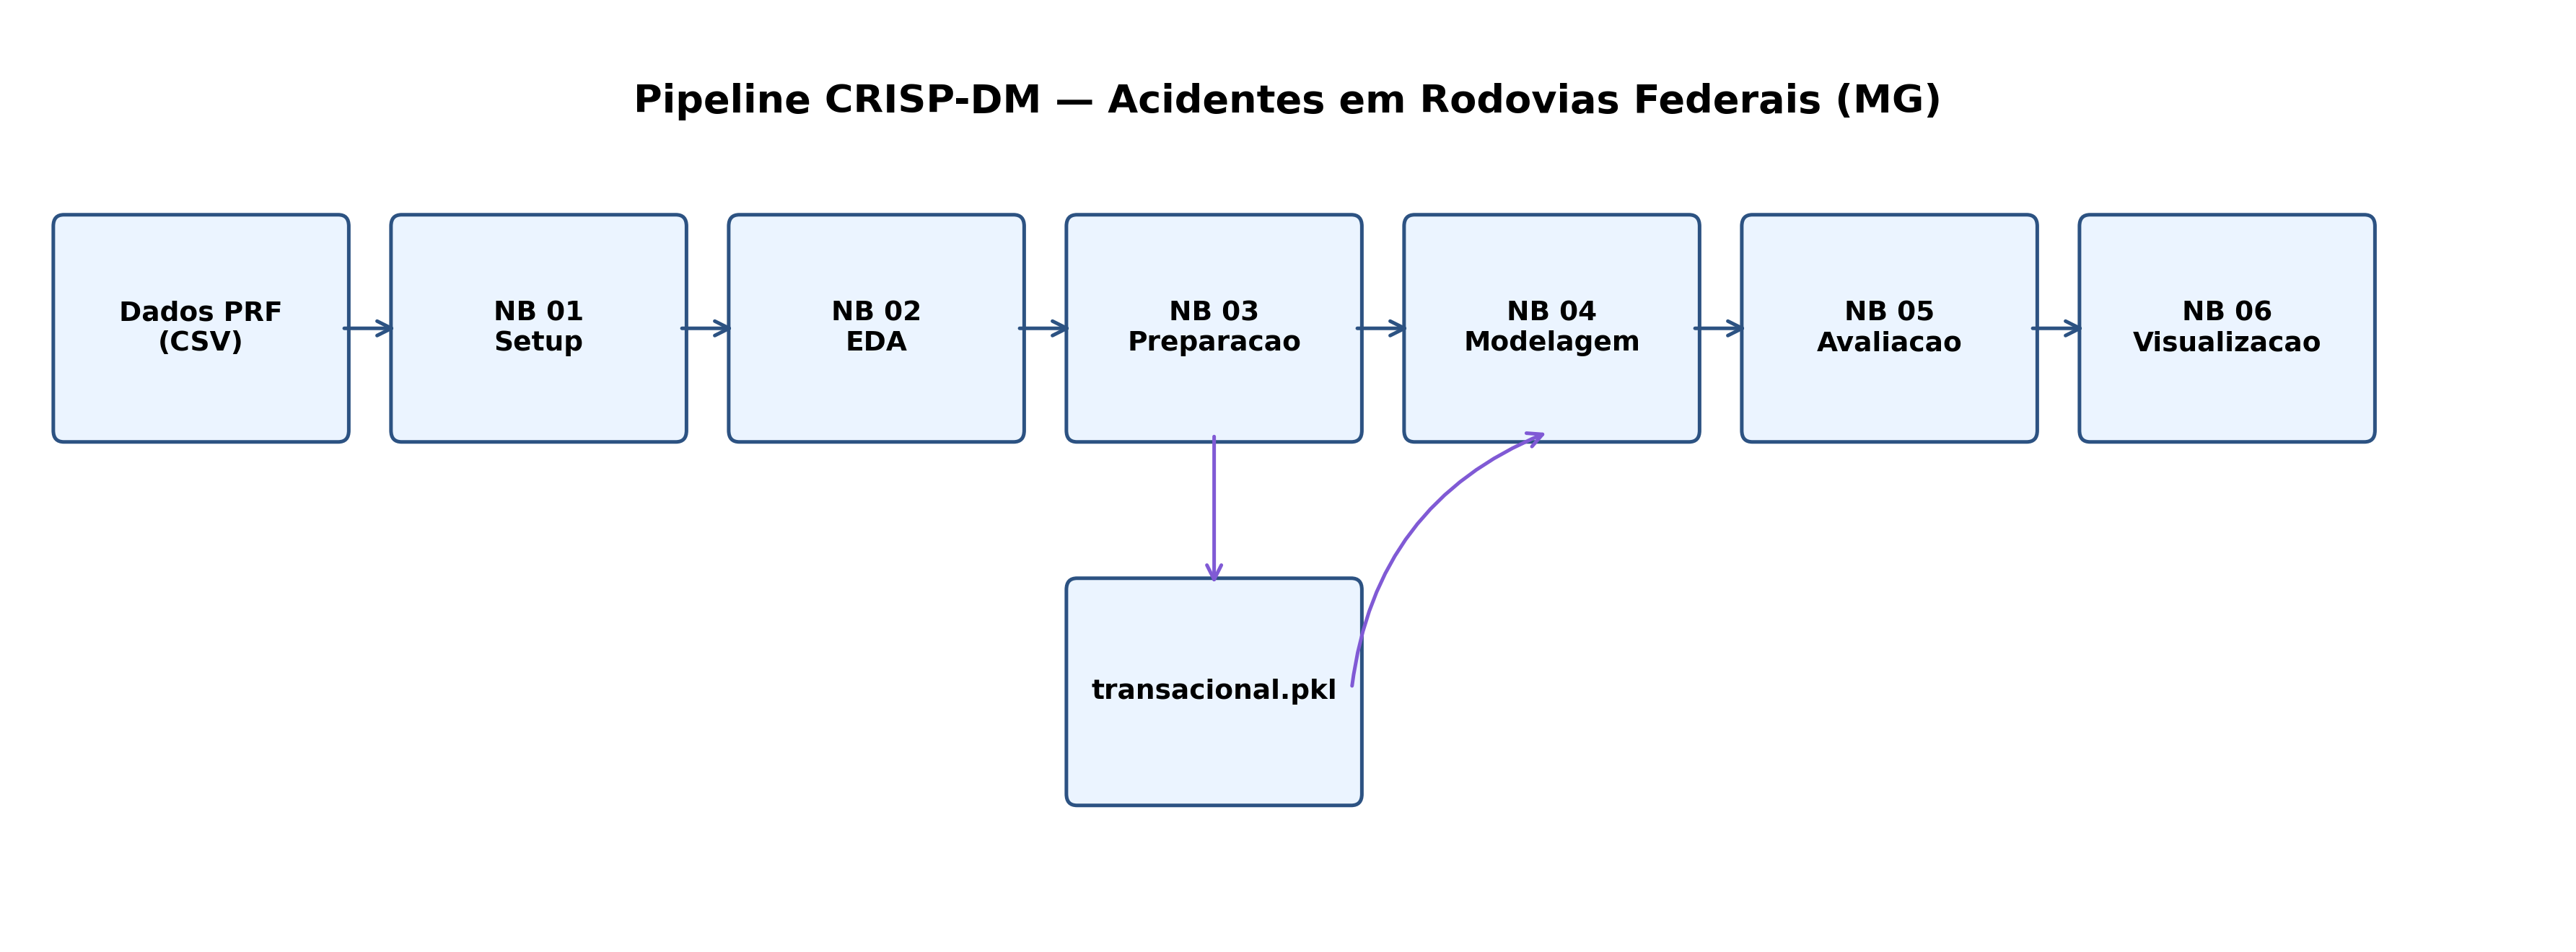
\includegraphics[width=\textwidth]{pipeline_crisp_dm.png}
    \caption{Pipeline CRISP-DM implementado: fluxo de dados da PRF até visualização.}
    \label{fig:pipeline}
\end{figure}

\subsection{Business \& Data Understanding --- Concluído}

Na fase de Business and Data Understanding, os notebooks \texttt{01\_setup\_e\_carregamento.ipynb} e \texttt{02\_analise\_exploratoria.ipynb} estabelecem a infraestrutura de carregamento e a compreensão inicial dos dados. O notebook~01 define o dicionário \texttt{DATASETS}, a variável \texttt{ACTIVE\_DATASET} e as funções reutilizáveis de carregamento e concatenação com filtro por UF, permitindo alternar entre as três granularidades disponíveis sem modificar o código analítico downstream.

O notebook~02 concentra a análise exploratória completa: avaliação de qualidade dos dados (valores ausentes e inconsistências), distribuições univariadas e bivariadas, análise temporal e geográfica, cálculo de Cramér's~V entre variáveis categóricas e gravidade, além da produção de 17 visualizações. Ao final desta fase, formulamos as hipóteses H1--H5 e documentamos implicações práticas para a mineração, como o impacto do desbalanceamento de classes sobre o suporte mínimo.

\subsection{Data Preparation --- Concluído}

A fase de Data Preparation, implementada no notebook \texttt{03\_preparacao\_dados.ipynb}, transforma o dataset bruto em uma representação adequada ao FP-Growth. Inicialmente, tratamos valores ausentes preenchendo categorias com ``Não Informado'' e padronizamos strings e a conversão numérica do campo \texttt{km}. Em seguida, criamos features derivadas --- \texttt{mes}, \texttt{faixa\_horaria}, \texttt{fim\_de\_semana}, \texttt{gravidade\_binaria} e \texttt{faixa\_km} --- que enriquecem a granularidade temporal e espacial da base.

A representação transacional converte cada ocorrência em um conjunto de itens binários no formato \texttt{coluna=valor}. Após a codificação one-hot, aplicamos filtragem de itens com frequência inferior a 1\% ou superior a 99\%, reduzindo a dimensionalidade de 207 para 83 itens. Os artefatos processados são persistidos em \texttt{data/processed/} (\texttt{df\_limpo.pkl} e \texttt{transacional.pkl}) para consumo pelos notebooks de modelagem e avaliação.

\subsection{Modeling --- Planejado}

A fase de Modeling será conduzida no notebook \texttt{04\_modelagem.ipynb}. A infraestrutura de mineração já foi montada e validada em execução piloto; os experimentos formais previstos incluem mineração global via FP-Growth sobre a base transacional completa, com \texttt{min\_support} calibrado a partir do desbalanceamento observado na EDA. A partir dos itemsets frequentes, geraremos regras de associação filtrando associações com lift superior a 1, ordenando-as por relevância e extraindo separadamente aquelas cujo consequente indica gravidade fatal.

Como etapa complementar, aplicaremos K-Means sobre atributos categóricos codificados e padronizados, determinando o número de clusters por meio do método do cotovelo e do silhouette score. A mineração será então repetida de forma independente em cada segmento, buscando capturar padrões locais que possam estar mascarados na análise global. Por fim, executaremos FP-Growth em janelas mensais para avaliar a estabilidade temporal dos padrões identificados.

\subsection{Evaluation --- Planejado}

A fase de Evaluation será distribuída entre os notebooks \texttt{05\_avaliacao\_ia\_responsavel.ipynb} e \texttt{06\_visualizacao\_resultados.ipynb}. Nela, consolidaremos tabelas comparativas das regras mais relevantes, traduziremos padrões selecionados para linguagem natural e analisaremos a estabilidade temporal das associações entre períodos distintos. Também incluiremos disclaimers explícitos sobre a distinção entre correlação e causalidade, além de produzir visualizações e exportações em formatos compatíveis com o relatório final (LaTeX, Markdown e figuras em alta resolução).

\section{Estratégia de Avaliação}

\subsection{Métricas de Regras de Associação}

Cada regra de associação $A \rightarrow B$ será avaliada por meio de métricas clássicas da literatura. O \textbf{suporte} mede a frequência conjunta de $A \cup B$ na base; a \textbf{confiança} expressa $P(B \mid A)$, indicando a probabilidade condicional do consequente dado o antecedente; e o \textbf{lift} compara a confiança observada com a esperada sob independência estatística, de modo que valores superiores a 1 indicam associação positiva. Complementarmente, \textbf{conviction} e \textbf{leverage} serão utilizados para detectar dependências assimétricas que podem passar despercebidas quando se considera apenas confiança e lift.

Além das métricas quantitativas, adotaremos critérios de seleção orientados à qualidade interpretativa das regras. Regras redundantes --- aquelas com o mesmo consequente e antecedentes sobrepostos --- serão removidas, priorizando-se padrões com antecedente de até três itens. Regras triviais, caracterizadas por lift próximo de 1 ou suporte extremo, serão excluídas para evitar a apresentação de associações estatisticamente fracas ou demasiadamente óbvias.

\subsection{Diretriz 1: Explicabilidade (Operacionalização Prevista)}

A diretriz de explicabilidade é pertinente neste projeto porque a mineração de regras de associação pode produzir um volume elevado de padrões, nem todos necessariamente úteis ou compreensíveis. No domínio de segurança viária, interpretações equivocadas --- como atribuir causalidade a uma simples coocorrência estatística --- podem levar a conclusões socialmente inadequadas. Por isso, os resultados precisam ser comunicados de forma clara, acompanhados de métricas e limitações explícitas.

A operacionalização prevista seguirá quatro passos integrados ao pipeline de avaliação. Primeiramente, filtraremos regras com antecedentes curtos (até três itens), favorecendo padrões de leitura direta. Em seguida, removeremos redundâncias, mantendo a formulação mais simples quando duas regras apresentarem confiança similar. Cada regra selecionada será traduzida para linguagem natural, acompanhada de suporte, confiança e lift. Por fim, incluiremos um disclaimer explícito de que associação estatística não implica relação causal.

Essa abordagem melhora a comunicabilidade dos resultados, mas impõe trade-offs relevantes. Ao priorizar simplicidade, corremos o risco de descartar padrões complexos potencialmente importantes; por isso, os critérios de filtragem deverão ser calibrados com cuidado para não eliminar associações substantivas.

\subsection{Diretriz 2: Monitoramento e Avaliação (Operacionalização Prevista)}

A diretriz de monitoramento e avaliação é pertinente porque os fatores associados à gravidade dos acidentes podem variar ao longo do tempo em resposta a mudanças de infraestrutura, legislação, fluxo de veículos e políticas de fiscalização. Uma regra identificada em determinado intervalo temporal pode, portanto, ser transitória e não generalizável a outros períodos.

Para incorporar essa diretriz, executaremos FP-Growth em janelas temporais mensais e compararemos os conjuntos de regras obtidos em cada período. Calcularemos a recorrência de cada regra ao longo dos meses e classificaremos os padrões como \textbf{estáveis} quando aparecerem em pelo menos 50\% dos períodos analisados, ou como \textbf{transitórios} quando surgirem em menos de 30\%. Para as regras estáveis, documentaremos a evolução de lift e confiança ao longo do tempo.

Essa estratégia torna a análise mais robusta frente a variações contextuais, mas aumenta a complexidade experimental. A subdivisão temporal reduz o volume de registros por janela, o que dificulta a identificação de padrões sobre acidentes fatais --- classe minoritária --- exigindo equilíbrio entre granularidade temporal e confiabilidade estatística.

\section{Plano de Experimentos}

\subsection{Experimento 1: Mineração Global e Grid de Parâmetros}

O primeiro experimento busca identificar itemsets frequentes e regras de associação globais, além de calibrar os hiperparâmetros da mineração. Para isso, variaremos sistematicamente \texttt{min\_support} em $\{0{,}01,\; 0{,}03,\; 0{,}05,\; 0{,}10\}$, \texttt{min\_confidence} em $\{0{,}3,\; 0{,}5,\; 0{,}7\}$ e \texttt{min\_lift} em $\{1{,}0,\; 1{,}5,\; 2{,}0\}$, totalizando 36 combinações. Para cada configuração, registraremos o número de itemsets, o número de regras geradas, a quantidade de regras associadas à gravidade e o tempo de execução do FP-Growth. As métricas de saída incluirão a distribuição de lift entre as regras retidas e o custo computacional por combinação de parâmetros.

\subsection{Experimento 2: Clustering + Mineração por Segmento}

O segundo experimento visa capturar padrões locais que possam estar mascarados na análise global. Após codificar os atributos categóricos e padronizá-los com StandardScaler, determinaremos o número de clusters $k$ por meio do método do cotovelo e do silhouette score, explorando $K \in [2, 9]$. Com o K-Means aplicado, executaremos FP-Growth de forma independente em cada segmento e compararemos as regras locais com as globais, investigando em particular a hipótese H5 sobre diferenças entre contextos urbanos e rurais.

\subsection{Experimento 3: Estabilidade Temporal}

O terceiro experimento avalia a robustez temporal das regras, em consonância com a diretriz de Monitoramento e Avaliação. A base será segmentada por mês a partir de \texttt{data\_inversa}, executando-se FP-Growth em cada janela com no mínimo 100 registros. Os conjuntos de regras serão então comparados entre períodos, classificando-se cada padrão quanto à estabilidade ou transitividade ao longo do tempo.

\subsection{Experimento 4: Visualizações e Exportação}

O quarto experimento consolida o material para o relatório final. Prevê-se a produção de pelo menos dez visualizações --- incluindo distribuição de suporte dos itemsets, ranking de regras por lift, scatter suporte$\times$confiança, rede de regras, evolução temporal e perfis de cluster --- em resolução de 300~dpi. Paralelamente, exportaremos tabelas de regras selecionadas em formatos LaTeX e Markdown, integrando-as à redação do documento final.

\section{Cronograma até 30/06/2026}

As fases de setup, análise exploratória e preparação dos dados (Fases 1--3 do CRISP-DM) foram concluídas entre abril e maio de 2026. O presente relatório de progresso consolida esse avanço e detalha o plano experimental para as etapas restantes. A Tabela~\ref{tab:cronograma} apresenta a distribuição das atividades previstas até a entrega do relatório final, em 30/06/2026.

\begin{table}[H]
    \centering
    \caption{Cronograma de execução restante.}
    \label{tab:cronograma}
    \begin{tabular}{lll}
        \toprule
        \textbf{Atividade} & \textbf{Período} & \textbf{Status} \\
        \midrule
        Setup, EDA e preparação (Fases 1--3) & Abr--Mai/2026 & Concluído \\
        Relatório de Progresso & Até 01/06/2026 & Em entrega \\
        Modelagem global + grid (Exp.~1) & 01--10/06/2026 & Planejado \\
        Clustering + mineração local (Exp.~2) & 10--15/06/2026 & Planejado \\
        Estabilidade temporal (Exp.~3) & 15--20/06/2026 & Planejado \\
        Avaliação IA responsável + visualizações (Exp.~4) & 20--25/06/2026 & Planejado \\
        Redação do Relatório Final & 25--30/06/2026 & Planejado \\
        \bottomrule
    \end{tabular}
\end{table}

\addcontentsline{toc}{section}{Referências}
\begin{thebibliography}{99}
    \bibitem{zaki2020} ZAKI, M. J.; MEIRA JR, W. \textit{Data Mining and Machine Learning: Fundamental Concepts and Algorithms}. 2nd ed. Cambridge University Press, 2020.
    \bibitem{wirth2000} WIRTH, R.; HIPP, J. CRISP-DM: Towards a standard process model for data mining. In: \textit{Proceedings of the 4th International Conference on the Practical Applications of Knowledge Discovery and Data Mining}, 2000.
    \bibitem{prf2026} BRASIL. Polícia Rodoviária Federal. \textbf{Dados Abertos da PRF}. Brasília, 2026. Disponível em: \url{https://www.gov.br/prf/pt-br/acesso-a-informacao/dados-abertos/dados-abertos-da-prf}.
\end{thebibliography}

\end{document}
